%% using aastex version 6.3
\documentclass[twocolumn]{aastex63}

%%%%%%%%%%%%%%%%%%%%%%%%%%%%%%%%%%%%%%%%%%%%%%%%%%%%%%%%%%%%%%%%%%%%%%%%%%%%%%%%
%%
%% The following section defines new commands for comments from co-authors
%%
\definecolor{DarkOrange}{RGB}{204, 85, 0}
\definecolor{LincolnGreen}{RGB}{17, 102, 0}
\definecolor{Rust}{HTML}{9B4F0F}
\definecolor{DarkCyan}{HTML}{008B8B}
\definecolor{MediumAquaMarine}{HTML}{66CDAA}


\def\ion#1#2{#1$\;${\footnotesize\rm{#2}}\relax}

\newcommand{\xander}[1]{{\color{red} XH: \textbf{#1}}}
\newcommand{\aam}[1]{{\color{DarkOrange} aam: \textbf{#1}}}

\newcommand{\todo}[1]{{\color{magenta} to-do: {#1}}}

\usepackage{lineno}
% \linenumbers
\usepackage{pifont}% http://ctan.org/pkg/pifont
\newcommand{\cmark}{\ding{51}}%
\newcommand{\xmark}{\ding{55}}%

\usepackage{multirow, amsmath}

%%
%%%%%%%%%%%%%%%%%%%%%%%%%%%%%%%%%%%%%%%%%%%%%%%%%%%%%%%%%%%%%%%%%%%%%%%%%%%%%%%%


%% Reintroduced the \received and \accepted commands from AASTeX v5.2
\received{\today}
\revised{}
\accepted{}
%% Command to document which AAS Journal the manuscript was submitted to.
%% Adds "Submitted to " the argument.
\submitjournal{}

%% For manuscript that include authors in collaborations, AASTeX v6.3
%% builds on the \collaboration command to allow greater freedom to 
%% keep the traditional author+affiliation information but only show
%% subsets. The \collaboration command now must appear AFTER the group
%% of authors in the collaboration and it takes TWO arguments. The last
%% is still the collaboration identifier. The text given in this
%% argument is what will be shown in the manuscript. The first argument
%% is the number of author above the \collaboration command to show with
%% the collaboration text. If there are authors that are not part of any
%% collaboration the \nocollaboration command is used. This command takes
%% one argument which is also the number of authors above to show. A
%% dashed line is shown to indicate no collaboration. This example manuscript
%% shows how these commands work to display specific set of authors 
%% on the front page.
%%
%% For manuscript without any need to use \collaboration the 
%% \AuthorCollaborationLimit command from v6.2 can still be used to 
%% show a subset of authors.
%
%\AuthorCollaborationLimit=2
%
%% will only show Schwarz & Muench on the front page of the manuscript
%% (assuming the \collaboration and \nocollaboration commands are
%% commented out).
%%
%% Note that all of the author will be shown in the published article.
%% This feature is meant to be used prior to acceptance to make the
%% front end of a long author article more manageable. Please do not use
%% this functionality for manuscripts with less than 20 authors. Conversely,
%% please do use this when the number of authors exceeds 40.
%%
%% Use \allauthors at the manuscript end to show the full author list.
%% This command should only be used with \AuthorCollaborationLimit is used.

%% The following command can be used to set the latex table counters.  It
%% is needed in this document because it uses a mix of latex tabular and
%% AASTeX deluxetables.  In general it should not be needed.
%\setcounter{table}{1}

%%%%%%%%%%%%%%%%%%%%%%%%%%%%%%%%%%%%%%%%%%%%%%%%%%%%%%%%%%%%%%%%%%%%%%%%%%%%%%%%
%%
%% The following section outlines numerous optional output that
%% can be displayed in the front matter or as running meta-data.
%%
%% If you wish, you may supply running head information, although
%% this information may be modified by the editorial offices.
\shorttitle{}
\shortauthors{}
%%
%% You can add a light gray and diagonal water-mark to the first page 
%% with this command:
%% \watermark{text}
%% where "text", e.g. DRAFT, is the text to appear.  If the text is 
%% long you can control the water-mark size with:
%% \setwatermarkfontsize{dimension}
%% where dimension is any recognized LaTeX dimension, e.g. pt, in, etc.
%%
%%%%%%%%%%%%%%%%%%%%%%%%%%%%%%%%%%%%%%%%%%%%%%%%%%%%%%%%%%%%%%%%%%%%%%%%%%%%%%%%
\graphicspath{{./}{figures/}}
%% This is the end of the preamble.  Indicate the beginning of the
%% manuscript itself with \begin{document}.

\begin{document}

\title{A Morphological Classification Model to Identify Unresolved PanSTARRS1 Sources II: Update to the PS1 Point Source Catalog}

%% LaTeX will automatically break titles if they run longer than
%% one line. However, you may use \\ to force a line break if
%% you desire. In v6.3 you can include a footnote in the title.

%% A significant change from earlier AASTEX versions is in the structure for 
%% calling author and affiliations. The change was necessary to implement 
%% auto-indexing of affiliations which prior was a manual process that could 
%% easily be tedious in large author manuscripts.
%%
%% The \author command is the same as before except it now takes an optional
%% argument which is the 16 digit ORCID. The syntax is:
%% \author[xxxx-xxxx-xxxx-xxxx]{Author Name}
%%
%% This will hyperlink the author name to the author's ORCID page. Note that
%% during compilation, LaTeX will do some limited checking of the format of
%% the ID to make sure it is valid. If the "orcid-ID.png" image file is 
%% present or in the LaTeX pathway, the OrcID icon will appear next to
%% the authors name.
%%
%% Use \affiliation for affiliation information. The old \affil is now aliased
%% to \affiliation. AASTeX v6.3 will automatically index these in the header.
%% When a duplicate is found its index will be the same as its previous entry.
%%
%% Note that \altaffilmark and \altaffiltext have been removed and thus 
%% can not be used to document secondary affiliations. If they are used latex
%% will issue a specific error message and quit. Please use multiple 
%% \affiliation calls for to document more than one affiliation.
%%
%% The new \altaffiliation can be used to indicate some secondary information
%% such as fellowships. This command produces a non-numeric footnote that is
%% set away from the numeric \affiliation footnotes.  NOTE that if an
%% \altaffiliation command is used it must come BEFORE the \affiliation call,
%% right after the \author command, in order to place the footnotes in
%% the proper location.
%%
%% Use \email to set provide email addresses. Each \email will appear on its
%% own line so you can put multiple email address in one \email call. A new
%% \correspondingauthor command is available in V6.3 to identify the
%% corresponding author of the manuscript. It is the author's responsibility
%% to make sure this name is also in the author list.
%%
%% While authors can be grouped inside the same \author and \affiliation
%% commands it is better to have a single author for each. This allows for
%% one to exploit all the new benefits and should make book-keeping easier.
%%
%% If done correctly the peer review system will be able to
%% automatically put the author and affiliation information from the manuscript
%% and save the corresponding author the trouble of entering it by hand.

\correspondingauthor{A.~A.~Miller}
\email{amiller@northwestern.edu}


%% Note that the \and command from previous versions of AASTeX is now
%% depreciated in this version as it is no longer necessary. AASTeX 
%% automatically takes care of all commas and "and"s between authors names.

%% AASTeX 6.3 has the new \collaboration and \nocollaboration commands to
%% provide the collaboration status of a group of authors. These commands 
%% can be used either before or after the list of corresponding authors. The
%% argument for \collaboration is the collaboration identifier. Authors are
%% encouraged to surround collaboration identifiers with ()s. The 
%% \nocollaboration command takes no argument and exists to indicate that
%% the nearby authors are not part of surrounding collaborations.

%% Mark off the abstract in the ``abstract'' environment. 
\begin{abstract}


\end{abstract}

%% Keywords should appear after the \end{abstract} command. 
%% See the online documentation for the full list of available subject
%% keywords and the rules for their use.
\keywords{}

%% From the front matter, we move on to the body of the paper.
%% Sections are demarcated by \section and \subsection, respectively.
%% Observe the use of the LaTeX \label
%% command after the \subsection to give a symbolic KEY to the
%% subsection for cross-referencing in a \ref command.
%% You can use LaTeX's \ref and \label commands to keep track of
%% cross-references to sections, equations, tables, and figures.
%% That way, if you change the order of any elements, LaTeX will
%% automatically renumber them.
%%
%% We recommend that authors also use the natbib \citep
%% and \citet commands to identify citations.  The citations are
%% tied to the reference list via symbolic KEYs. The KEY corresponds
%% to the KEY in the \bibitem in the reference list below. 

\section{Introduction} \label{sec:intro}

\todo{Make sure the idea of an alert packet is well defined and consistent throughout}

The proliferation of wide-field time-domain surveys over the past $\sim$decade
has led to the discovery of a bevy of novel extragalactic transients
\citep[e.g.,][]{quimby11,Gezari12,Gal-Yam14,Abbott17a,Prentice18,
IceCube-Collaboration18}. While these wide-field surveys have been enabled by
significant advances in detector technology, software has proven equally
important \citep[e.g.,][]{Masci17,Masci19,Smith20,Jones20} as many of these
critical discoveries have been facilitiated by the rapid identification and
dissemination of new transient candidates in near real time
\citep[e.g.,][]{Patterson19}.

Reliable catalogs identifying stars and galaxies, or similarly unresolved and
resolved sources, are an essential cog in the machinery necessary to identify
extragalactic transients. On a nightly basis, time-domain sureys are inundated
with transient candidates, the vast majority of which are considered ``bogus''
\citep{Bloom12}. Despite sophisticated software capable of whittling down the
number of likely transients by several orders of magnitude
\citep[e.g.,][]{Brink13,Goldstein15,Duev19,Smith20}, the number of candidates
still vastly outpaces the spectroscopic resources necessary to classify
everything that varies \citep[e.g.,][]{Kulkarni20}. The aforementioned
star--galaxy catalogs therefore play an essential role in the search for
extragalactic transients by removing candidates that are associated with
stellar-like objects that are therefore likely to be Galactic in origin.

To this end we previously created the PanSTARRS-1 Point Source Catalog
\citep[PS1 PSC; Tachibana \& Miller 2018, hereafter ][]{Tachibana18}, which
provides probabilistic point-source like classifications for $\sim$1.5 billion
sources detected by PanSTARRS-1 \citep[PS1;][]{Chambers16}. This catalog has
been deployed by the Zwicky Transient Facility \citep[ZTF;][]{Bellm19} and
other surveys \citep{Smith20,Moller20} to identify likely extragalactic
transients. The PS1 PSC has been demonstrated to be an important ingredient in
the systematic search for extragalactic transients \citep{Fremling20,De20}.

\todo{??? Add quick explanation of mean, forced, and stack phot from PS1 ???}

A downside to the PS1 PSC is that it does not provide classifications for
sources that are not ``detected'' in the PS1 \texttt{StackObjectThin} table
\citep[the definition of a PS1 stack detection is given in][]{Tachibana18}. Of
the $\sim$3.5 billion sources in the PS1 \texttt{stackObjectThin} table, the
vast majority of the $\sim$2 billion missing from the PS1 PSC are either
spurious or have an extremely low signal-to-noise ratio (S/N), such that the
methods in \citet{Tachibana18} would not provide a reliable classification.
There are an additional 144,870,754 high-S/N
sources missing from the PS1 PSC because they have multiple entries in the PS1
\texttt{StackObjectThin} table with $\mathtt{primaryDetection} =
1$.\footnote{The \texttt{primaryDetection} flag identifies which entry within
the PS1 \texttt{stackObjectThin} table was detected from the stack image that
provides the best coverage with minimal projection stretching. Roughly 0.5\%
of the \texttt{stackObjectThin} sources have multiple rows with
$\mathtt{primaryDetection} = 1$, effectively making it impossible to identify
which row should be used in conjunction with the model from
\citet{Tachibana18}.} These sources, many of which are moderately bright
stars, have an $\mathtt{sg_score} = 0.5$ within the ZTF alert packets, i.e.,
there classification is ambiguous, and as a result stars can end up in
extragalactic transient streams.

\todo{Add note about ~1.92 B sources in ZTF PS1 table???}

Here, we present an update to the PS1 PSC by classifying these
144,870,754 sources using photometry from the
\texttt{ForcedObjectMean} table in the PS1 database. While we previously
showed that the PS1 forced photometry does not separate resolved and
unresolved sources with the same fidelity as its stack photometry
\citep{Tachibana18}, we can, using a nearly identical methodology as
\citet{Tachibana18}, nevertheless achieve similar performance with the PS1
forced photometry. We apply our new model to the \todo{$\sim$140; need final
number} million previously unclassified sources, providing a new and useful
supplement to the PS1 PSC.\footnote{During the preparation of this manuscript
\citet{Beck20} published a new machine learning catalog (PS1-STRM) to separate
the $\sim$3.5 billion sources in the PS1 \texttt{ForcedMeanObject} table. The
main difference between the PS1 PSC and PS1-STRM is the training set used by
each machine learning model, which we discuss in more detail below.}

\section{Model Data and PS1 Features}

\todo{better section title}

The methodology adopted here is extremely similar to the one presented in
\citep{Tachibana18}. The only major difference between the two is the feature
set used in the construction of the machine learning model. We discuss this
difference below, followed by a brief summary of the model construction.

\todo{Add note about the FoM}

\subsection{Training Set}

As a training set for the model, we use deep observations of the COSMOS field
from the \textit{Hubble Space Telescope} (\textit{HST}). The superior
resolution of \textit{HST} enables reliable morphological classifications for
sources as faint as $\sim$25\,mag \citep{Leauthaud07}. There are 80,867 bright
\textit{HST} sources from \citet{Leauthaud07} that have PS1 counterparts
\citep[within a 1\arcsec match radius; see][]{Tachibana18} in the
\texttt{ForcedMeanObject} table (see \S\ref{sec:features}). Of those, the
47,825 PS1 sources with $\mathtt{nDetections} \ge 1$ are adopted as the
training set for our model. For this model the training set is $\sim$1.6\%
larger than that used in \citet{Tachibana18} because more HST/COSMOS sources
are detected, using our version of a ``detection'', via PS1 forced photometry
than PS1 stack photometry.

\subsection{PS1 Forced Photometry Features}\label{sec:features}

Regardless of the choice of algorithm, the basic goal of a machine learning
model is to build a map between source features, numerical and/or categorical
properties that can be measured for an individual source, and labels, the
target output, often a classification, of the model. This mapping is learned
via a training set, a subset of the data with known labels, afterwhich the
model can classify any source based on its features.

In \citet{Tachibana18} we introduced the concept of ``white flux'' features,
whereby measurements in the five individual PS1 filters ($g_\mathrm{PS1}$,
$r_\mathrm{PS1}$, $i_\mathrm{PS1}$, $z_\mathrm{PS1}$, $y_\mathrm{PS1}$) were
summed, via a weighted mean, to produce a ``total'' flux or shape measurement
across all filters.\footnote{Only filters in which the source is detected,
i.e., the flux is $> 0$, are included in the sum.} Machine learning models are
limited by their training sets: there is no guarantee that their empirical
mapping will correctly extend beyond the boundaries enclosed by the training
set. Given the significant systematic uncertainties associated with Galactic
reddening, and the tendancy for spectroscopic samples, which are typically
used to define training sets, to be biased in their target selection
\citep[see e.g.,][]{Miller17}, the motivation for ``white flux'' features
becomes clear: they reduce potential biases in the final classifications due
to select effects in how the training set sources were targeted. Therefore, as
in \citet{Tachibana18}, we use ``white flux'' features in this study.

The PS1 \texttt{StackObjectAttributes} table provides both flux and shape
(e.g., second moment of the radiation intensity) measurements in each of the
five PS1 filters, whereas the \texttt{ForcedMeanObject} table only provides
flux measurements.\footnote{The \texttt{ForcedMeanObject} table provides
average measurements across all epochs on which a PS1 source is observed, and
the average second moment of the radiation intensity is somewhat meaningless
as the orientation of the detector and observing conditions vary image to
image.} Morphological classification models, such as the one presented here,
are somewhat hindered by the lack of shape information in the
\texttt{ForcedMeanObject} table \citep[see for example the different shape
features in Figure~2 of][]{Tachibana18}. 

To create the feature set for our machine learning model, we create ``white
flux'' features for the six different flux measurements available in the
\texttt{ForcedMeanObject} table (\texttt{FPSFFlux}, \texttt{FKronFlux},
\texttt{FApFlux}, \texttt{FmeanflxR5}, \texttt{FmeanflxR6},
\texttt{FmeanflxR7}), as well as the \texttt{E1} and \texttt{E2} measurements,
which represent the mean polarization parameters from \citet{Kaiser95}. As in
\citet{Tachibana18}, we use flux ratios, rather than the raw flux
measurements, which provide morphological classifications that are independent
of S/N \citep{Lupton01}.

\begin{figure*}
    \centering
    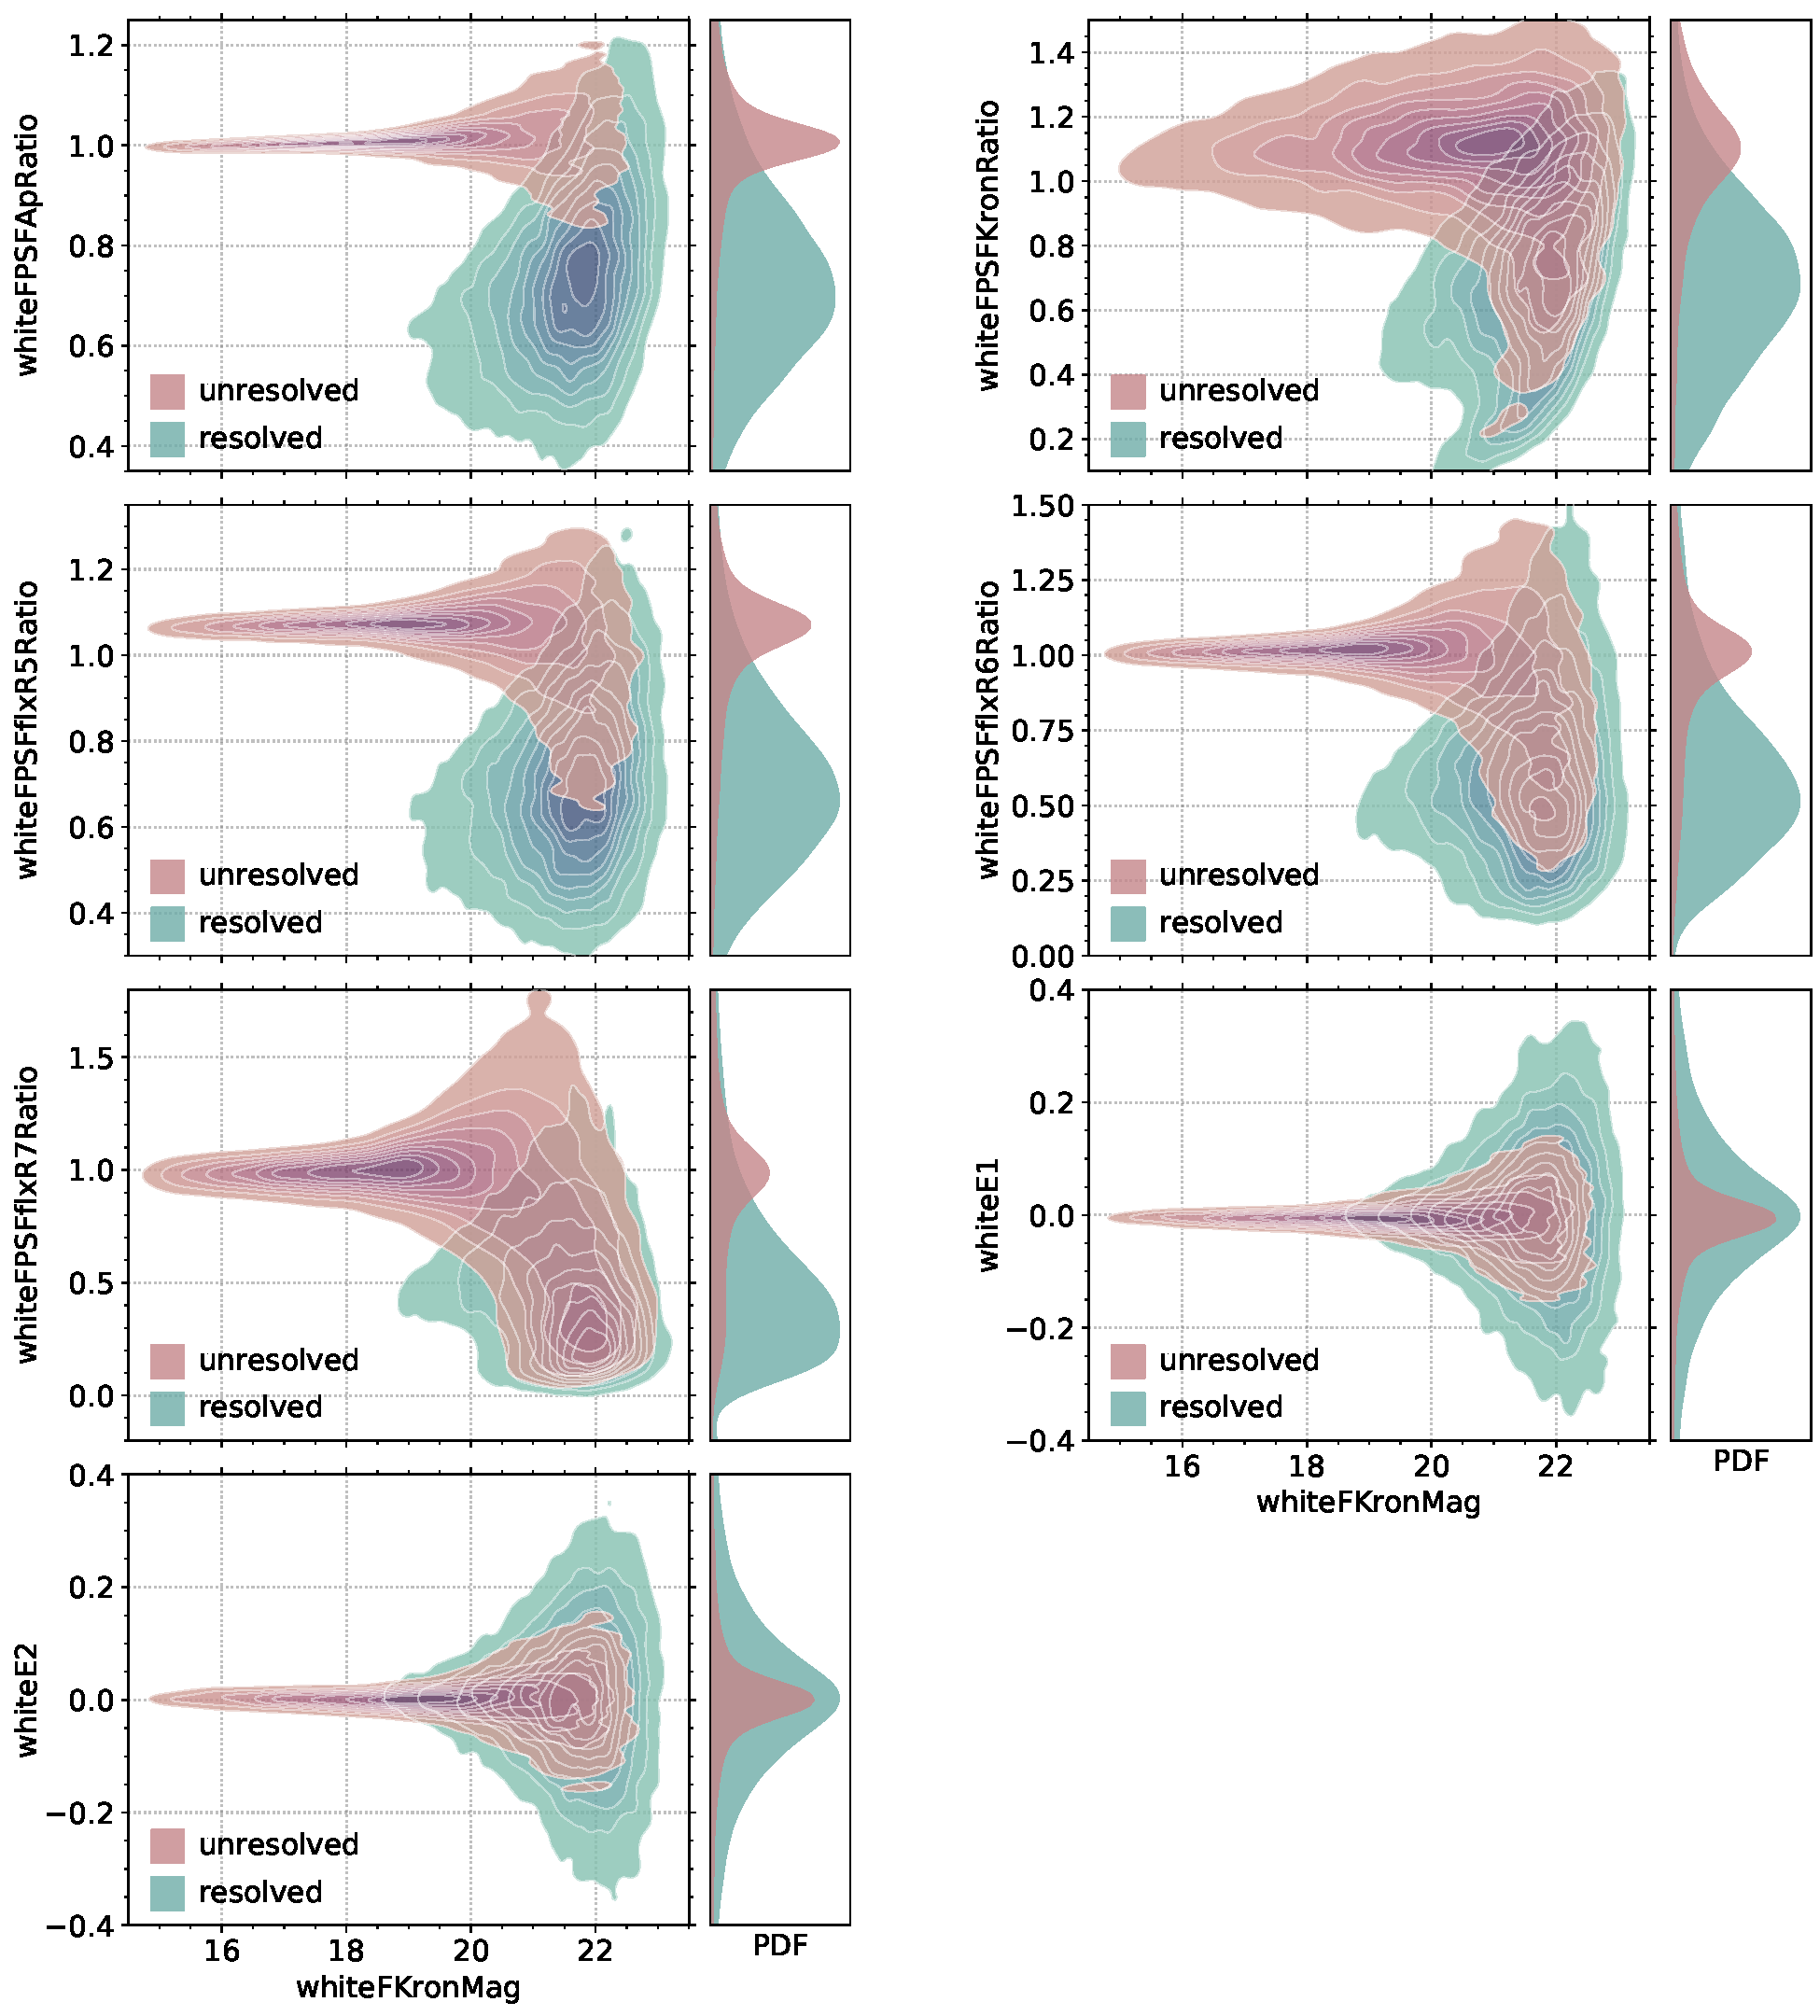
\includegraphics[width=6.5in]{./figures/whiteFeatures.pdf}
    %
    \caption{The primary square panels show Gaussian KDEs of the PDF for each
    of the ``white flux'' features as a function of \texttt{whiteFKronMag}
    ($=-2.5\log_{10}[\mathtt{whiteFKronFlux}/3631]$) for all sources in the
    training set. Unresolved point sources are shown via the red-purple
    contours, while resolved, extended objects are shown via blue-green
    contours. The shown contour levels extend from 0.9 to 0.1 in 0.1
    intervals. To the right of each primary panel is a marginalized 1D KDE of
    the PDF for the individual features, where the amplitudes of the KDEs have
    been normalized by the relative number of point sources and extended
    objects.}
    %
    \label{fig:features}
\end{figure*} 

Our final model includes nine features, five flux ratios:\\
$\mathtt{whiteFPSFApRatio} = \mathtt{whiteFPSFlux/whiteFApFlux}$,
$\mathtt{whiteFPSFKronRatio} = \mathtt{whiteFPSFlux/whiteFKronFlux}$,
$\mathtt{whiteFPSFFflxR7Ratio} = \mathtt{whiteFPSFlux/whiteFFflxR7Flux}$,
$\mathtt{whiteFPSFFflxR7Ratio} = \mathtt{whiteFPSFlux/whiteFFflxR7Flux}$,
$\mathtt{whiteFPSFFflxR7Ratio} = \mathtt{whiteFPSFlux/whiteFFflxR7Flux}$, the
white polarization parameters: \texttt{whiteE1} and \texttt{whiteE2}, and two
``simple'' distance measures: \texttt{whiteFPSFKronDist} and
\texttt{whiteFPSFKronDist} (see \S\ref{sec:simple_model}). The distribution of
these features for stars and galaxies in the training set is shown in
Figure~\ref{fig:features}.

\subsection{The ``Distance'' Features}\label{sec:simple_model}

In \citet{Tachibana18} we introduced a ``simple'' model to classify sources
based solely on their measured \texttt{whitePSFFlux} and
\texttt{whiteKronFlux}. The model was inspired by the use of flux ratios,
which have been shown to provide a good discriminant between resolved and
unresolved sources \citep[e.g., the SDSS morphological \texttt{CLASS}
parameter][]{Lupton01}. At moderate to low S/N, however, flux ratios no longer
provide accurate classifications (see e.g., Figure~\ref{fig:features}). The
simple model from \citet{Tachibana18} leverages this fact by measuring the
distance of each source from a line drawn in the
\texttt{whitePSFFlux}--\texttt{whiteKronFlux} plane. Unlike a flux ratio, the
simple model preserves information about the S/N, meaning sources with large
absolute distances from the dividing line can be classified with greater
confidence.

Following from Equation~3 in \citet{Tachibana18}, ``simple'' features can be
calculated as:
%
\begin{multline}
 \mathtt{whiteFlux1Flux2Dist}(a) = \\
 \frac{\mathtt{whiteFlux1} - a\times\mathtt{whiteFlux2}}{ \sqrt{1 + a^2}},
 \label{eqn:simple_feat}
\end{multline}
%
where \texttt{whiteFlux1} and \texttt{whiteFlux2} are ``white flux''
measurements introduced in \S\ref{sec:features} (e.g.,
\texttt{whiteFKronFlux}), $a$ is the slope of the line in the
texttt{whiteFlux1}--\texttt{whiteFlux2} plane, and
\texttt{whiteFlux1Flux2Dist} is the orthogonal distance of a source from the
line. For this study we construct two simple features for inclusion in our
machine learning model: \texttt{whiteFPSFFKronDist} and
\texttt{whiteFPSFFApDist}.

We determine the optimal value of $a$ for the simple features via cross
validation. We find $a = 0.7512$ for the \texttt{whiteFPSFFKronDist} feature
and $a = 0.7784$ for the \texttt{whiteFPSFFApDist} feature maximizes the FoM.
Empirically \texttt{whiteFPSFFApDist} is better at separating resolved and
unresolved sources than \texttt{whiteFPSFFKronDist}, and therefore the
``simple'' model, discussed below, is based on \texttt{whiteFPSFFApDist}. The
\texttt{whiteFPSFFApDist} and \texttt{whiteFPSFFKronDist} distribution of
resolved and unresolved sources is shown in Figures~\ref{fig:psf_ap} and
\ref{fig:psf_kron}, respectively.

\begin{figure}
    \centering
    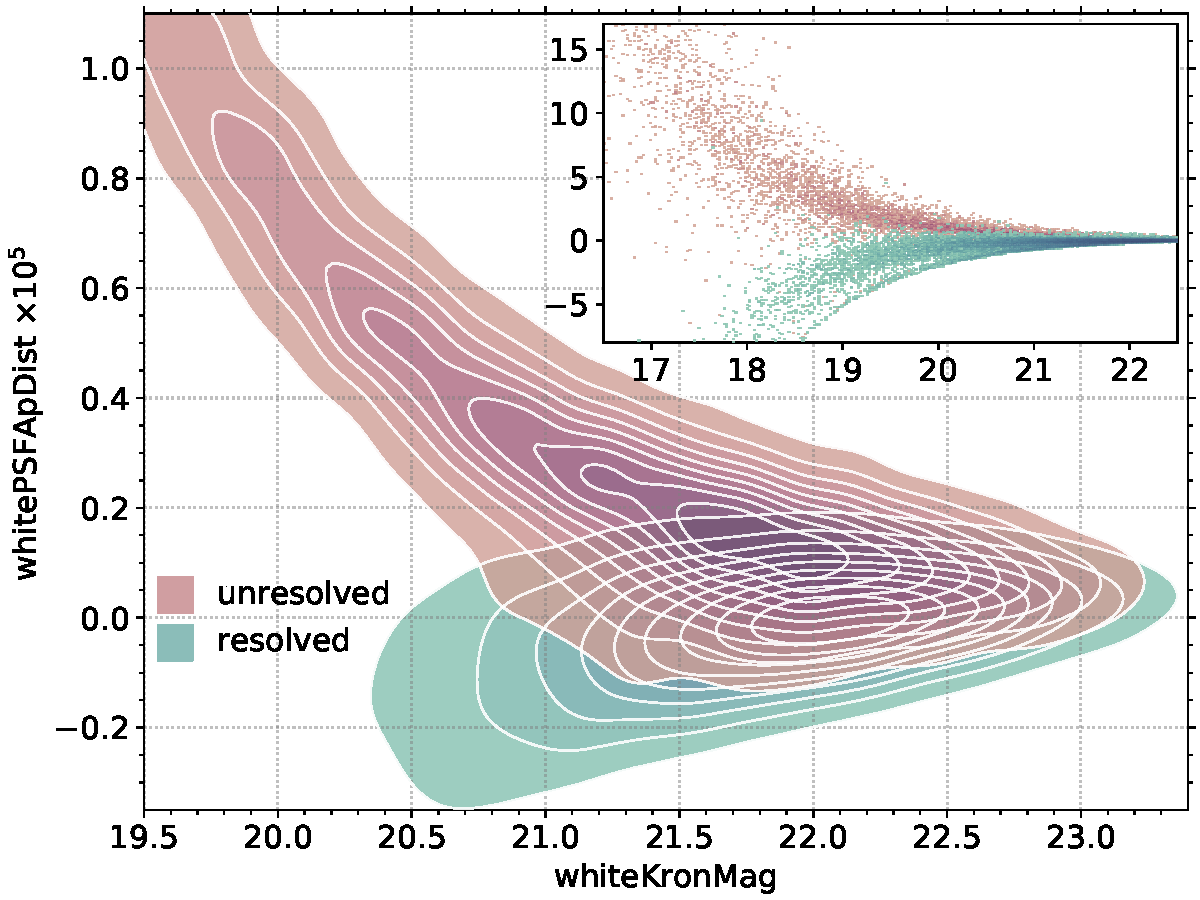
\includegraphics[width=\columnwidth]{./figures/whiteFPSFApDist.pdf}
    %
    \caption{The distribution of $\mathtt{whitePSFKronDist}$ values for HST
    training set point sources (labeled stars) and extended objects (labeled
    galaxies) as a function of \texttt{whiteKronMag}. The colors and contours
    are the same as Figure~\ref{fig:features}. The horizontal dashed line
    shows the optimal threshold ($\mathtt{whitePSFKronDist} \ge 9.2 \times
    10^{-7}$) for resolved--unresolved classification. The upper-right inset
    shows a zoom-out highlighting the stark difference between stars and
    galaxies at the bright end.}
    %
    \label{fig:psf_ap}
\end{figure}

\begin{figure}
    \centering
    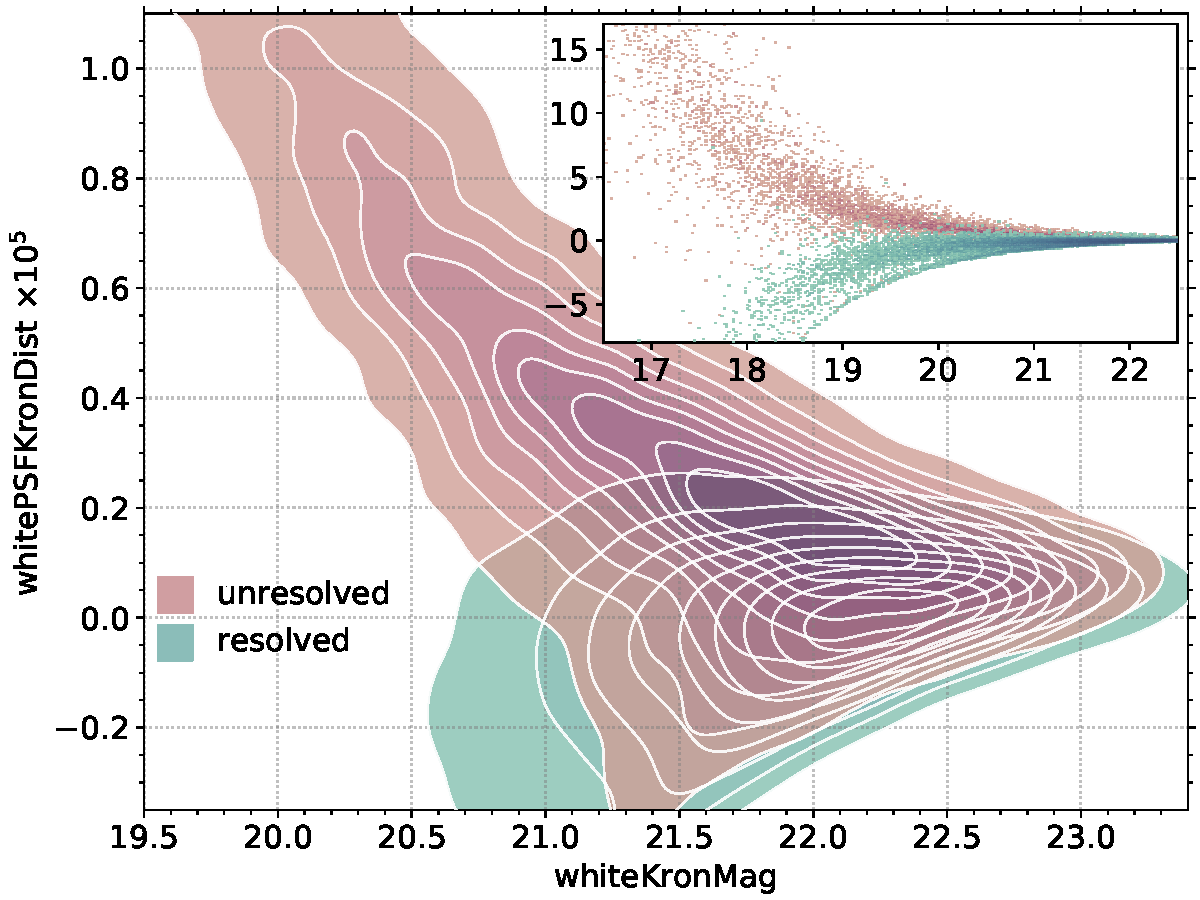
\includegraphics[width=\columnwidth]{./figures/whiteFPSFKronDist.pdf}
    %
    \caption{Same as Figure~\ref{fig:psf_ap}, but showing the distribution for
    \texttt{whiteFPSFKronDist}.}
    %
    \label{fig:psf_kron}
\end{figure}  

\subsection{Model Construction}

Using the nine features mentioned in \S\ref{sec:features}, we use the random
forest (RF) algorithm \citep{Breiman01}, as implemented in
\texttt{scikit-learn} \citep{Pedregosa11}, to classify PS1 sources as resolved
or unresolved. Briefly, the RF algorithm constructs an ensemble of decision
trees \citep{Breiman84}, where each tree is constructed using a bootstrapped
sample of the training set \citep[a method known as ``bagging'';][]{Breiman96}
and the split for each branch within the tree is selected from a random subset
of full feature set. The result is a lower variance estimator than is possible
from a single decision tree.

To train the RF model, we replicate the procedure in \citet{Tachibana18}. We
use $k$-fold cross validation (CV) to optimize the model tuning parameters,
namely the number of trees in the forest $N_\mathrm{tree}$, the random number
of features for splitting at each node $m_\mathrm{try}$, and the minimum
number of sources in a terminal leaf of the tree $\mathtt{nodesize}$. Our CV
procedure utilizes both an inner and outter loop, each with $k = 10$ folds. In
the inner loop, a $k = 10$ folds CV grid search is performed over the three
tuning parameters, while predictions from the optimal grid location are
applied to the 1/10 of the training set that was withheld in the outer loop.
This process is then repeated for the remaining 9 folds in the outer loop. We
adopt the average results from the 10 different grid searches to arrive at
optimal model parameters of: \xander{help me fill in these values}. The RF
model results are not strongly dependent on the final choice of tuning
parameters.

\section{Results}

Our aim is to maximize the FoM of the RF model. We show receiver operating characteristic (ROC) curves of the RF,
simple, and PS1\footnote{The PS1 model is defined by a single hard cut on the
PSF--Kron flux ratio measured in the $i_\mathrm{PS1}$ band \citep[for further
details see][]{Tachibana18}.} models in Figure~\ref{fig:hst_roc}. From
Figure~\ref{fig:hst_roc}, it is clear that the RF and simple models greatly
outperform the PS1 model. Furthermore, while the gains are modest, the
inclusion of all the ``white flux'' features and use of machine learning is
justified as the RF model produces a higher FoM than the simple model.

\begin{figure}[t]
 \centering
  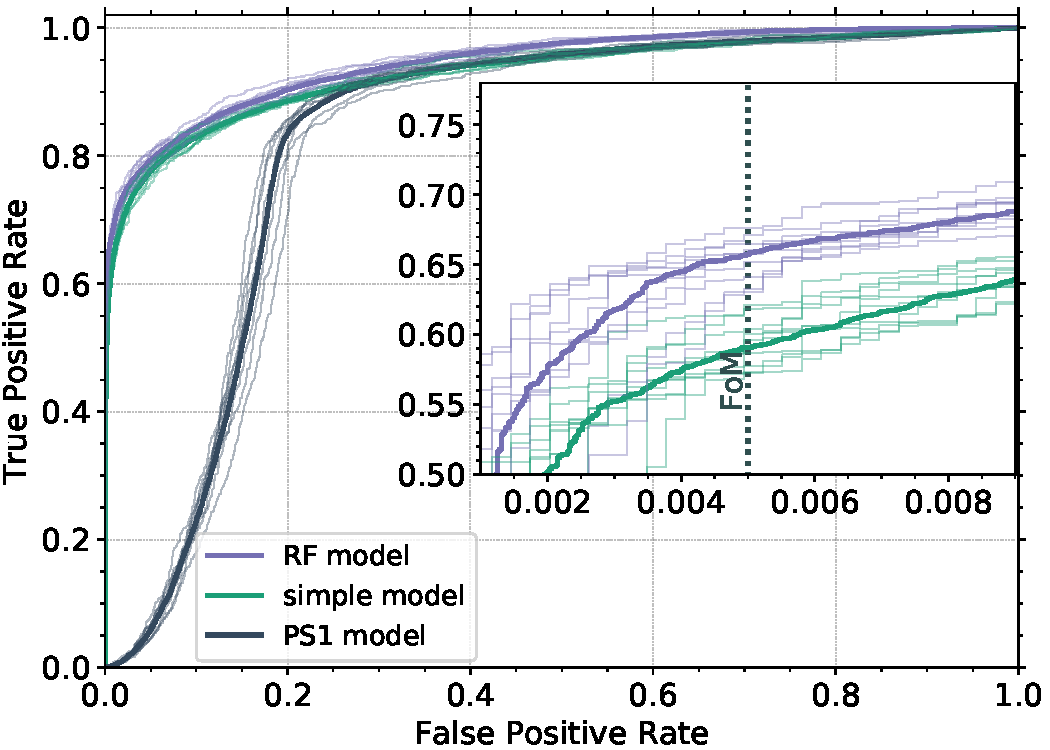
\includegraphics[width=\columnwidth]{./figures/CV_ROC_FHST.pdf}
  %
  \caption{ ROC curves comparing the relative performance of the PS1, simple,
  and RF models for HST sources with $i_\mathrm{PS1}$ detections. The thick,
  solid slate gray, green, and purple lines show the ROC curves for the PS1,
  simple, and RF models, respectively. The light, thin lines show the ROC
  curves for the individual CV folds. The inset on the right shows a zoom in
  around FPR = 0.005, shown as a dotted vertical line, corresponding to the
  FoM (the PS1 model is not shown in the inset, because it has very low FoM).
  \xander{The inset needs to be adjusted to a yrange of $\sim$0.45--0.72 -
  also whiteFKronMag}}
  %
  \label{fig:hst_roc}
\end{figure}

The FoM of each of the three models considered here is summarized in
Table~\ref{tbl:hst_cv}. In addition to providing largest FoM, the RF model is
also the most accurate of the three and it has the largest area under the ROC
curve (ROC AUC). We robustly conclude that, of the models considered here, the
RF model is best. Comparing with Table~1 in \citet{Tachibana18}, we find that
the forced-photometry features derived in this study do not provide the same
discriminating power as the PS1 stack-photometry features used in
\citet{Tachibana18}. The use of the forced-photometry features results in a
FoM that is $\sim$7\% worse than the stack-photometry features. We discuss the
implications of this in \S\ref{sec:discussion}. This slight reduction in
performance is countered by the fact that we can classify $\sim$140 million
additional sources using the forced-photometry features.

\begin{deluxetable}{cccc}
    \tablecolumns{4} 
    \tablewidth{0pt} 
    \tablecaption{ CV Results for the Training Set \label{tbl:hst_cv}}
    \tablehead{ 
    \colhead{model} & \colhead{FoM} & \colhead{Accuracy} & \colhead{ROC AUC}
    }
    \startdata
    RF & \textbf{0.657} $\pm$ 0.016 & \textbf{0.918} $\pm$ 0.003 & \textbf{0.945} $\pm$ 0.003 \\
    simple & 0.591 $\pm$ 0.017 & 0.887 $\pm$ 0.007 & 0.930 $\pm$ 0.003 \\
    PS1 & 0.002 $\pm$ 0.001 & 0.809 $\pm$ 0.008 & 0.827 $\pm$ 0.009 \\
    \enddata
    \tablecomments{Uncertainties represent the sample standard deviation for the 10 individual folds used in CV.}
\end{deluxetable}

We show the CV accuracy of the RF, simple, and PS1 models in
Figure~\ref{fig:hst_acc}. As in \citet{Tachibana18}, we find that the RF
model provides more accurate classifications than the alternatives.

\begin{figure}[t]
 \centering
  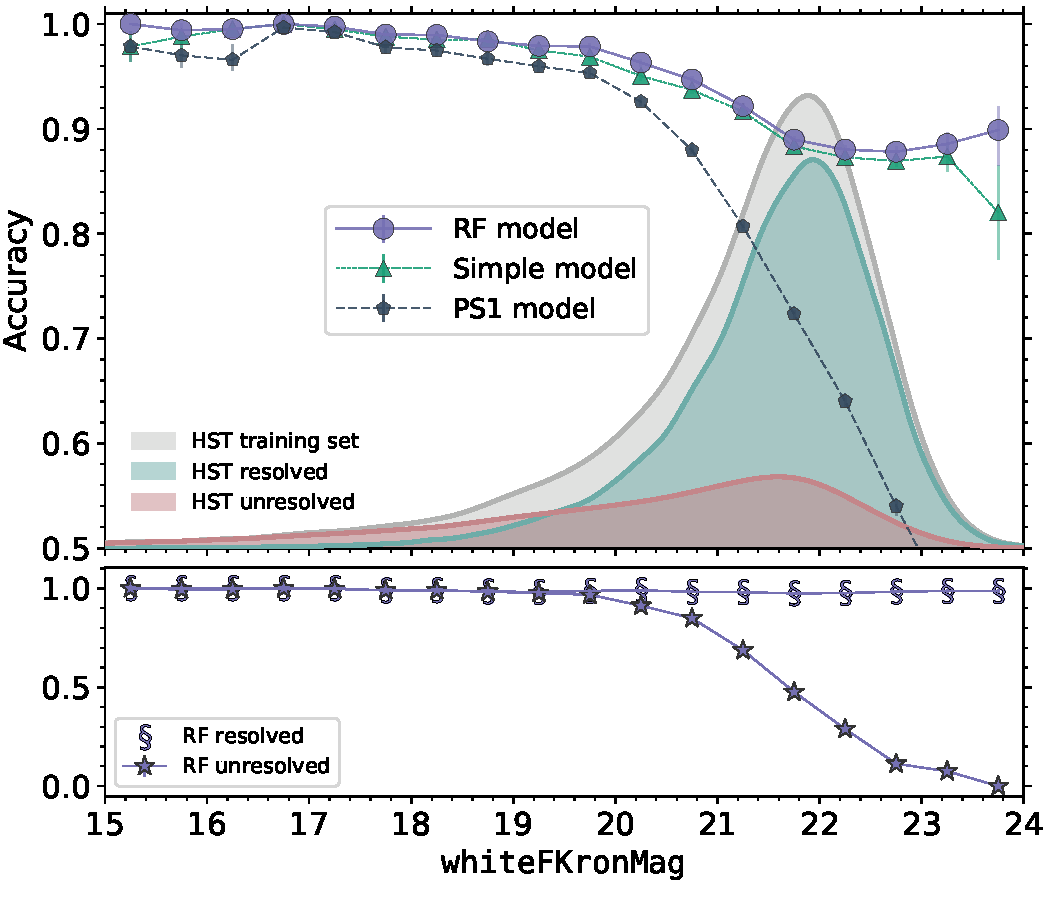
\includegraphics[width=\columnwidth]{./figures/CV_Accuracy_FHST.pdf}
  %  
  \caption{Model accuracy as a function of \texttt{whiteFKronMag} for HST
  sources with $i_\mathrm{PS1}$ detections. Accuracy curves for the PS1,
  simple and RF models are shown as slate gray pentagons, green triangles, and
  purple circles, respectively. The bin widths are 0.5\,mag, and the error
  bars represent the 68\% interval from bootstrap resampling. Additionally, a
  Gaussian KDE of the PDF for the training set, as well as the unresolved
  point sources and resolved, extended objects in the same subset is shown in
  the shaded gray, red, and green regions, respectively. The amplitude of the
  star and galaxy PDFs have been normalized by their relative ratio compared
  to the full $i_\mathrm{PS1}$-band subset. \xander{Need to update legend to
  say resolved and unresolved respectively - should probably udpate the
  symbols too - also whiteFKronMag}}
  %
  \label{fig:hst_acc}
\end{figure}  

As expected, the accuracy of each model shown in Figure~\ref{fig:hst_acc}
decreases with the S/N. The accuracy curve for the RF model features a slight
departure from expectation in that is is nearly flat for \texttt{whiteKronMag}
between $\sim$22 and 24\,mag. \todo{Need to confirm this argument is indeed
correct} This quasi-plateau in the RF model accuracy can be understood as the
result of two components of the training set: (i) unresolved sources
completely dominate the source counts at these magnitudes, and (ii) the
well-defined locus of unresolved sources in the training set (see
Figure~\ref{fig:features}) becomes heavily blended with the resolved source
population at these brightness levels. Taken together the model will be biased
towards classifying all faint sources as resolved, and with \todo{NNN}\% of
the $\mathtt{whiteKronMag} > 22.5$\,mag training set sources being unresolved,
a plateau in accuracy of $\sim$87\% makes sense. This is confirmed in
Figure~\ref{fig:sg_accuracy}, which shows the true positive rate (TPR) for
both resolved and unresolved sources as a function of \texttt{whiteKronMag}. A
near 100\% TPR for faint resolved sources combined with a few correctly
classified unresolved sources leads to observed quasi-plateau in
Figure~\ref{fig:hst_acc}.

\begin{figure}
    \centering
    \includegraphics[width=\columnwidth]{./figures/CV_sg_mag_accuracy.pdf}
    %
    \caption{}
    %
    \label{fig:sg_accuracy}
\end{figure}    

\subsection{The Updated PS1 PSC Catalog}\label{sec:ps1psc_update}

Following the construction of the RF model that utilizes PS1 forced photometry
features, we can provide morphological classifications for the PS1 sources
that are currently missing from the PS1 PSC. Of the $\sim$426 million
``missing'' sources, $\sim$144 million have PS1 DR2 \texttt{ForcedMeanObject}
photometry that pass our detection criteria (see \ref{app:cat_counts} for more
details). A histogram showing the distribution of the RF classification score
for these newly classified sources is shown in Figure~\ref{fig:psc_update}.

\begin{figure}
    \centering
    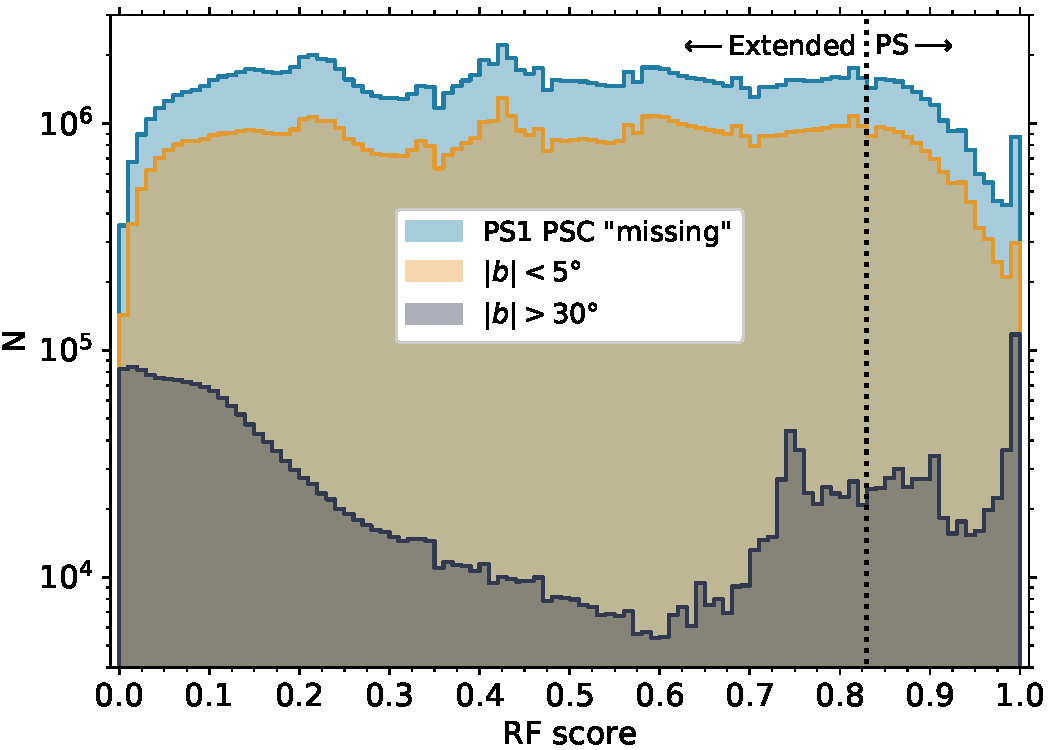
\includegraphics[width=\columnwidth]{./figures/PS1_PSC_update_hist.pdf}
    %
    \caption{Histogram showing the RF classification scores for the $\sim$144
    million newly classified sources from PS1. All of the newly classified
    sources are shown in blue, while Galactic plane sources ($|b| <
    5^{\circ}$) are shown in orange, and high galactic latitude sources ($|b|
    > 30^{\circ}$) are shown in grey. The vertical dotted line shows the
    conservative classification threshold adopted in \citet{Tachibana18}
    (sources to the right of the line are considered point sources). The vast
    majority of the newly classified sources are in the Galactic plane.}
    %
    \label{fig:psc_update}
\end{figure}    

Figure~\ref{fig:psc_update} shows that there are relatively few
high-confidence classifications (i.e., very likely extended sources with RF
score $\approx 0$ or very likely point sources with RF score $\approx 1$)
among the ``missing'' sources. Figure~\ref{fig:psc_update} also reveals the
likely explanation for this outcome: the vast majority of the newly classified
sources are in the Galactic plane. Of the $\sim$144 million newly classified
sources, $\sim$57\% have galactic latitude $\lvert b \rvert < 5$\,deg, while
$> 95$\% are in the Galactic plane ($\lvert b \rvert < 15$\,deg). The HST
COSMOS field, from which we derive our training set, has $b \approx 42$\,deg
and as a result includes very few stellar blends, which are common at low
galactic latitudes. The PS1 PSC also has significantly lower confidence
classifications in the Galactic plane \citep[see Figure~8 in][]{Tachibana18}.
That these sources were not ``detected'' in the PS1 stack images also suggests
that it is difficult to make reliable photometric measurements using the PS1
data, which could also contribute to the lower confidence classifications. The
upcoming third data release from the space-based \textit{Gaia} telescope
\citep{Perryman01} will improve this situation by classifying many of these
ambiguous sources as stars via parallax and proper motion measurements.

Ultimately, this update to the PS1 PSC has identified 17,945,494 likely point
sources using the optimized threshold from \citet[][RF score $\ge
0.83$]{Tachibana18}. While this number is small compared to the $\sim$734
million point sources in the original PS1 PSC, these $\sim$18 million newly
identified point sources would otherwise pass filters looking for
extragalactic transients in the ZTF alert stream. Their removal will reduce
the number of false positive transient candidates.

\todo{Get source counts on nDetections for things still not classified?}

\section{Deployment in the ZTF Real-Time Pipeline}\label{sec:discussion}

The ZTF real-time pipeline \citep{Masci19} provides AVRO alert packets
\citep[see][]{Patterson19} containing information (e.g., flux, position,
nearest neighbors) about any newly discovered sources of variability. The
packets include morphological classifications, based on the PS1 PSC
\citep{Tachibana18}, for the three closest PS1 sources within 30\arcsec\ of
the position of the newly observed variable source (see ~\ref{app:cat_counts}
for a summary of the PS1 sources included). As previously discussed, $\sim$426
million PS1 sources in the ZTF \texttt{Stars} table are not classified in the
original PS1 PSC.

Moving forward, ZTF alert packets now include the $\sim$144 million additional
classifications presented in \S\ref{sec:ps1psc_update}. \todo{Add sentence
from Frank about how these are designated} The addition of these new
classifications to the ZTF AVRO packets should not affect existing
alert-stream filters, as we describe below.

\input{./tables/thresholds.tex}

While a one-to-one mapping of point-source classification scores cannot be
made between \citet{Tachibana18} and this study, the similarity between the
two methodologies leads to classifications that are highly similiar.
Table~\ref{tbl:thresh} summarizes the TPR and FPR for different classfication
thresholds using the model from \citet{Tachibana18} and the RF model created
in this study. Table~\ref{tbl:thresh} shows that the PS1 stack photometry used
in \citet{Tachibana18} consistently produces a higher TPR, by $\sim$6--8\%,
than the PS1 forced photometry. The PS1 forced photometry used in this study
does have a lower FPR than \citet{Tachibana18} for all but the most liberal
point-source classification cuts. Thus, applying classification cuts developed
for the original PS1 PSC will ultimately lead to a higher TPR, as previously
unclassified point sources can now be removed from the stream, without
experiencing an overall increase in the FPR. As a result, we conclude that the
vast majority of users will not experience any significant change in the
results to their filters, aside from a slight reduction in false negatives
(stars that are classified as galaxies), following the update to the ZTF
\texttt{Stars} table.

\section{Discussion}

\section{Conclusions}

\acknowledgments

\vspace{5mm}
\facilities{}

%% Similar to \facility{}, there is the optional \software command to allow 
%% authors a place to specify which programs were used during the creation of 
%% the manuscript. Authors should list each code and include either a
%% citation or url to the code inside ()s when available.

\software{\texttt{astropy} \citep{Astropy-Collaboration13,
Astropy-Collaboration18}, 
          \texttt{scipy} \citep{2020SciPy-NMeth},
          \texttt{matplotlib} \citep{Hunter07}, 
          \texttt{pandas} \citep{McKinney10},
          \texttt{scikit-learn} \citep{Pedregosa11}}

\appendix

\section{The ZTF--PS1 Morphological Catalog}\label{app:cat_counts}

The ZTF database contains a table (\texttt{Stars}) with sources selected from
the PS1 DR1 that are used to provide morphological classifications in the ZTF
alert packets. The ZTF \texttt{Stars} table was seeded from the PS1
\texttt{MeanObject} table and includes all PS1 \texttt{MeanObject} sources
with $\mathtt{nDetections} \ge 3$.\footnote{Immediately after the release of
PS1 DR1 it was recommended that sources detected on at least three individual
PS1 images were unlikely to be spurious. Hence, the use of this selection cut
for the ZTF \texttt{Stars} table.} There are 1,919,106,844 sources in the ZTF
\texttt{Stars} table. Of these, 1,484,281,394 are classified in the PS1 PSC
and another 8,520,167 are classified as point sources based on \textit{Gaia}
parallax and/or proper motion measurements \citep{Tachibana18}. Therefore,
there are 426,305,283 sources in the ZTF \texttt{Stars} table that did not
meet the quality cuts necessary to be included in the PS1 PSC.\footnote{Only
sources with a single row designated as the \texttt{primaryDetection} in the
PS1 \texttt{StackObjectAttributes} table and a stack ``detection''
\citep[i.e., the PSF, Kron, and aperture flux are all $>0$ in at least one
filter, see][]{Tachibana18} are included in the PS1 PSC. }

For the $\sim$426 million ZTF \texttt{Stars} table sources not in the PS1 PSC,
5,885,633 had multiple rows in the PS1 \texttt{StackObjectAttributes} table
with $\mathtt{primaryDetection} = 1$, while the rest were not ``detected'' in
the PS1 stacks. As described in \S\ref{sec:ps1psc_update}, 144,870,754 of the
previously ``missing'' sources pass our \texttt{ForcedMeanObject}
``detection'' criteria (see \S\ref{}) and are now included in the PS1 PSC. 

The remaining $\sim$281 million sources do not have reliable photometry in
either the PS1 forced or stack tables, and as a result remain in the ZTF
\texttt{Stars} table with an ambiguous score of 0.5. It is worth noting that
$\sim$8\% of those $\sim$281 million are sources that were present in PS1 DR1,
and hence included in the ZTF \texttt{Stars} table, but are not present in PS1
DR2 (mostly because they have declination $\delta < -30$\,deg).\footnote{See
\url{https://outerspace.stsci.edu/display/PANSTARRS/PS1+DR2+caveats\#PS1DR2caveats-Missingdata} for more information.} Furthermore, $\sim$34\% of these
$\sim$281 million sources have $\mathtt{nDetections} = 3$, and $\sim$55\% have
$\mathtt{nDetections} \le 5$. That these sources have so few detections in PS1
increases the probability that they may be spurious, and even if they are not
spurious, they are otherwise very low S/N detections, which do not produce
highly confident classifications.

% 22524277 are at dec < -30


\bibliographystyle{aas_arxiv.bst}
\bibliography{/Users/adamamiller/Documents/tex_stuff/papers}

%% Include this line if you are using the \added, \replaced, \deleted
%% commands to see a summary list of all changes at the end of the article.
%\listofchanges

\end{document}

% End of file `sample63.tex'.
